%----------------------------------------------------------------------------
\chapter{Eredmények ismertetése és összefoglalás}
%----------------------------------------------------------------------------

\section{Különböző architektúrák összehasonlítása}

A nagyobb modellek pontosabb eredményeket és alacsonyabb WER-t értek el adatbázistól függetlenül. Viszont ez az idő drasztikus növekedésével járt együtt. 12x1-es architektúra nagyjából 5 millió paramétert, míg a 15x5-ös architektúra 18.9 millió paramétert használt. Futtatási idő esetén ez azt eredményezte, hogy fele annyi epoch-hoz másfélszer annyi időre volt szüksége, ami 3-szoros sebesség csökkenést eredményez. Következtetésképp lehetőség szerint érdemes minél több erőforrással dolgozni, az idő csökkentése végett és a mélyebb háló útján elindulni a precízebb végeredmény céljából.

\begin{figure}[!ht]
\centering
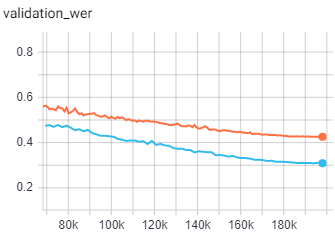
\includegraphics[width=100mm, keepaspectratio]{figures/architecture_12x1_vs_15x5.png}
\caption{15x5-ös - narancs és 12x1-es - kék architektúrák.}
\end{figure}

A 6.1-es ábrán látható viszont a mélyebb, összetettebb háló előnye, hiszen ekvseebb epoch alatt pontosabb eredményeket, alacsonyabb validation WER értéket sikerült elérni vele, mint a 12x1 architektúrával.

\section{Véletlenszerűen inicializált vs transfer learning}

Minden esetben megállapítható, hogy a transfer learning nagyban javította az elért eredményeket, annak ellenére, hogy az átvett modell súlyai egy másik ábécével, másik nyelven lettek tanítva.  Látható, hogy az emberek által generált hangok, a nyelvek struktúrája és logikája erősen összefügg.

\begin{figure}[!ht]
\centering
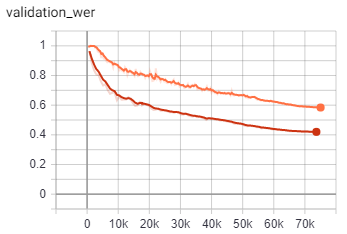
\includegraphics[width=100mm, keepaspectratio]{figures/12x1_pretrained_vs_random.png}
\caption{12x1-es architektúrák validation WER étékei pretrained - vörös és random inicializált - narancs súlyokkal.}
\end{figure}

\section{Mozilla Common Voice és Radio2}

A két adatbázis fő különbsége az adatok mennyisége volt. A Radio2-ből nagyjából 200 órányi adatot használtam fel, míg a Mozilla Common Voice-ból 45 órányit. Emiatt a Radio2-vel hosszabb tanításokra, de jobb általános eredményekre lehetett számítani.

Ennek megfigyelésére a két különböző adatbázison tanított modellek teljesítményét kell megvizsgálni. A Mozilla Common Voice adathalmazon tanított modell ~29\%-al jobb WER eredményt ért el a Radio2 adathalmazon tanított modellnél a Mozilla Common Voice-hoz tartozó teszt adathalamzon. Viszont a Radio2-ből leválasztott teszt adathalmazon lényegsebb, ~37\% körüli érték volt az eltérés a Radio2 adathalmazon tanult adatok javára. Látható, hogy a nagyobb adatmennyiség egy általánosabban jobban teljesítő modellt eredményezett.

\section{Javítási lehetőségek}

A jobb WER eredmények végett alkalmazhatóak a neurális hálók esetén a gyakran használt augmentációs módszerek. Ezek az elérhető hanganyag mennyiséget dúsítják fel különböző módszerekkel. Ez lehet az eredeti hanganyag torzítása, levágása, zaj hozzáadása vagy sebességének módosítása.

Nagyobb adatbázisok alkalmazása jobb általánosítást eredményez, ami a validációs WER érték csökkenésével jár együtt. Érdemes a különböző adatbázisokat összefogni és akár több ezer órányi adaton tanítani.

A sebesség növeléséhez a NeMo toolkit több lehetőséget is kínál. Az egyik a Mixed Precision\footnote{Mixed Precision lehetőség magyarázat az NVIDIA oldalán: \url{https://docs.nvidia.com/deeplearning/nemo/neural_mod_bp_guide/index.html}}, a másik módszer több GPU bevonása a tanítási folyamatba. Utóbbi esetben több, előre meghatározott GPU közt osztódik el az adat és kerül gyorsabb kiértékelésre.

Lehetséges még a tanítóadat pontos behatárolása. Mivel tanítás közben, a tanítási batch-ekbe különböző hosszúságú hangfájlok kerülnek betöltésre, így például egy 16-os batch méret esetén a GPU hamar kiértékeli az 5 másodperc hosszú hangfájlokat, de nem tud tovább haladni, míg a leghosszabbat, például egy 14 másodperceset nem értékelt ki. Ezen probléma elkerülése, és a GPU jobb kihasználása végett célszerű nagyjából egyforma hosszúságú adatokat felhasználni a tanításhoz.

Természetesen javulást eredményezhet a hiperparaméterekkel való kísérletezés, azok finomítása. Különböző adatok, nyelvek vagy architektúrák más-más paraméterekkel működnek jobban, nincsenek bevett számok, legfeljebb megközelítőleg.

\section{Végső gondolatok}

A beszédfelismerés már régóta velünk van, de egyre inkább elterjed és bekerül a köztudatba, mindennapjainkba a pontosság növekedésének következtében. Ehhez nagyban hozzájárul a klasszikus HM-től eltérő, napjainkban egyre inkább felkapott megközelítés a mély neuron háló alapú, end-to-end beszédfelismerés. Egyre több toolkit, és platform jelenik meg, amelyek könnyítik a neurális hálókkal való munkát, azok fejlesztését.

Az angoltól eltérő nyelvű automatikus beszédfelismerő rendszerek fejlesztése és kutatása fontos terület, hiszen a különböző nemzetek polgárai a saját nyelvükön akarnak beszélni. Segítséget nyújthatnak ebben a folyamatban a precíz, angol nyelvű modellek a transfer learning által, aminek következtében drasztikus javulás érhető el az új modell WER pontosságánál.

A nap mint nap megjelenő újabb architektúrák implementálásával a pontosság tovább növelhető, így korábban elképzelhetetlen, az embernél is nagyobb pontosságú beszédfelismerés valósítható meg, mely az élet számos területén használható fel.